% !TEX TS-program = XeLaTeX
% !TEX encoding = UTF-8 Unicode

\chapter{CSI 数据表示与特征处理}
\label{chap:features}
\defaultfont

\section{CSI 数据结构}
WiFi CSI 数据记录了无线信道在时间、频率和空间链路上的变化。对于包含多根发射天线和接收天线的采集设备，CSI 可表示为一个多维复数矩阵。矩阵中的每个元素对应某一时刻、某一子载波和某一发射接收天线链路上的信道响应。

设 CSI 序列包含 $T$ 个时间帧、$S$ 个子载波、$R$ 根接收天线和 $M$ 根发射天线，则 CSI 数据可表示为
\begin{equation}
X_{\mathrm{csi}}\in \mathbb{C}^{T\times S\times R\times M}.
\end{equation}
其中，时间维度反映人体姿态变化过程中的连续扰动；子载波维度反映不同频率分量下的信道差异；接收天线和发射天线维度反映不同空间传播链路上的信号变化。

\section{人体姿态对无线信道的影响}
室内无线传播通常由直达、反射、绕射和散射等多条路径共同构成。接收端观测到的信道响应可以概括为静态环境分量、人体相关分量和测量噪声之和：
\begin{equation}
H(f,t)=H_{\mathrm{s}}(f)+H_{\mathrm{h}}(f,t)+N(f,t),
\end{equation}
其中 $H_{\mathrm{s}}(f)$ 表示墙体、家具和固定设备形成的相对稳定传播分量，$H_{\mathrm{h}}(f,t)$ 表示人体对无线信号产生的遮挡、反射和散射分量，$N(f,t)$ 表示测量噪声及其他未建模扰动。

人体姿态发生变化时，躯干表面的空间位置、朝向和有效反射区域随之改变，部分传播路径的长度和衰减也会发生变化。由于接收信号是多条路径的复数叠加，即使人体整体位置基本不变，身体形态变化仍可能改变 CSI 的幅度和相位分布。但这种关系并不是一一对应的：环境布局、人与收发设备的相对位置以及个体体型均可能产生相似或更强的信道变化。因此，CSI 姿态检测需要利用多帧、多子载波和多天线链路的联合统计规律，而不能将某个单一测量值直接解释为脊柱结构信息。

\section{幅度与相位特征}
CSI 是复数形式，其幅度和相位分别表示为
\begin{equation}
H=Ae^{j\phi},
\end{equation}
其中 $A$ 为幅度，$\phi$ 为相位。幅度描述接收信号能量变化，相位描述信号传播过程中的相对偏移。人体姿态不同会造成信号传播路径和多径叠加方式不同，因此幅度和相位均包含姿态相关信息。

在实际采集中，幅度特征通常较为稳定，但容易受到距离、遮挡和发射功率变化影响；相位特征对细微路径变化更加敏感，但同时也更容易受到硬件偏移和噪声影响。因此，本文重点采用相位校正后的相对相位特征作为脊柱姿态检测的重要输入。

\section{原始相位误差模型}
理想条件下，CSI 相位反映传播路径造成的相位变化；实际测量相位还会叠加载波频率偏移、采样时钟偏移、包检测延迟和射频链路初始相位等误差。对于第 $s$ 个子载波和第 $r$ 条接收链路，测量相位可抽象表示为
\begin{equation}
\hat{\phi}_{s,r}(t)=\phi_{s,r}(t)+\phi_{\mathrm{c}}(t)+\phi_{\mathrm{d},s}(t)+b_r+\eta_{s,r}(t),
\end{equation}
其中 $\phi_{s,r}(t)$ 为与传播信道有关的相位，$\phi_{\mathrm{c}}(t)$ 为多条链路共享的公共偏移，$\phi_{\mathrm{d},s}(t)$ 为与子载波相关的误差项，$b_r$ 为接收链路的相对初始偏移，$\eta_{s,r}(t)$ 为随机噪声。

如果直接将 $\hat{\phi}_{s,r}(t)$ 输入分类器，模型可能把设备状态或采样误差作为类别依据。相位处理的目标不是恢复无法直接观测的绝对真实相位，而是通过相对关系削弱公共误差，并保留与人体扰动有关的链路差异。基于多天线复数比值的表示正是基于这一思路构造。

\section{接收天线相位比特征}
相位比特征通过不同接收天线之间的 CSI 复数比值构造。设 $H_{t,s,r,m}$ 表示第 $t$ 个时间帧、第 $s$ 个子载波、第 $r$ 根接收天线和第 $m$ 根发射天线对应的 CSI。本文以第 0 根接收天线为参考，对其他接收天线计算复数比值：
\begin{equation}
R_{t,s,r,m}=\frac{H_{t,s,r,m}}{H_{t,s,0,m}+\varepsilon},
\quad r=1,\ldots,R-1,
\end{equation}
其中 $\varepsilon$ 为防止分母为零的极小常数。相位比由复数比值的幅角得到：
\begin{equation}
\theta_{t,s,r,m}=\arg(R_{t,s,r,m}).
\end{equation}
该比值保留了不同接收天线链路之间的相对变化关系，并削弱了一部分公共相位偏移。随后沿时间维度对相位序列进行展开：
\begin{equation}
\tilde{\theta}_{t,s,r,m}=\operatorname{unwrap}(\theta_{t,s,r,m}).
\end{equation}
经过相位展开后，相邻时间帧之间由相位周期性造成的跳变被平滑处理，特征序列能够更稳定地表达人体姿态引起的无线信道变化。

若两条接收链路共享近似的公共相位项，则复数比值的幅角近似等于两条链路传播相位之差，公共项在相减过程中被部分抵消。但链路独立噪声、参考链路低幅度和天线硬件差异仍然存在，因此需要避免将相位比理解为无噪声特征。实际处理时应检查非有限值、异常幅度和序列长度，并保证训练与检测阶段使用相同的参考链路及维度顺序。

图~\ref{fig:csi_signal_example} 给出了数据集中一个正常姿态文件的实际 CSI 片段。幅度热图展示了 30 个子载波随时间的共同变化；相位比曲线则说明原始角度受 $[-\pi,\pi)$ 周期限制会出现跳变，沿时间维度展开后可获得连续轨迹，为后续差分与分位数统计提供稳定输入。

\begin{figure}[htbp]
\centering
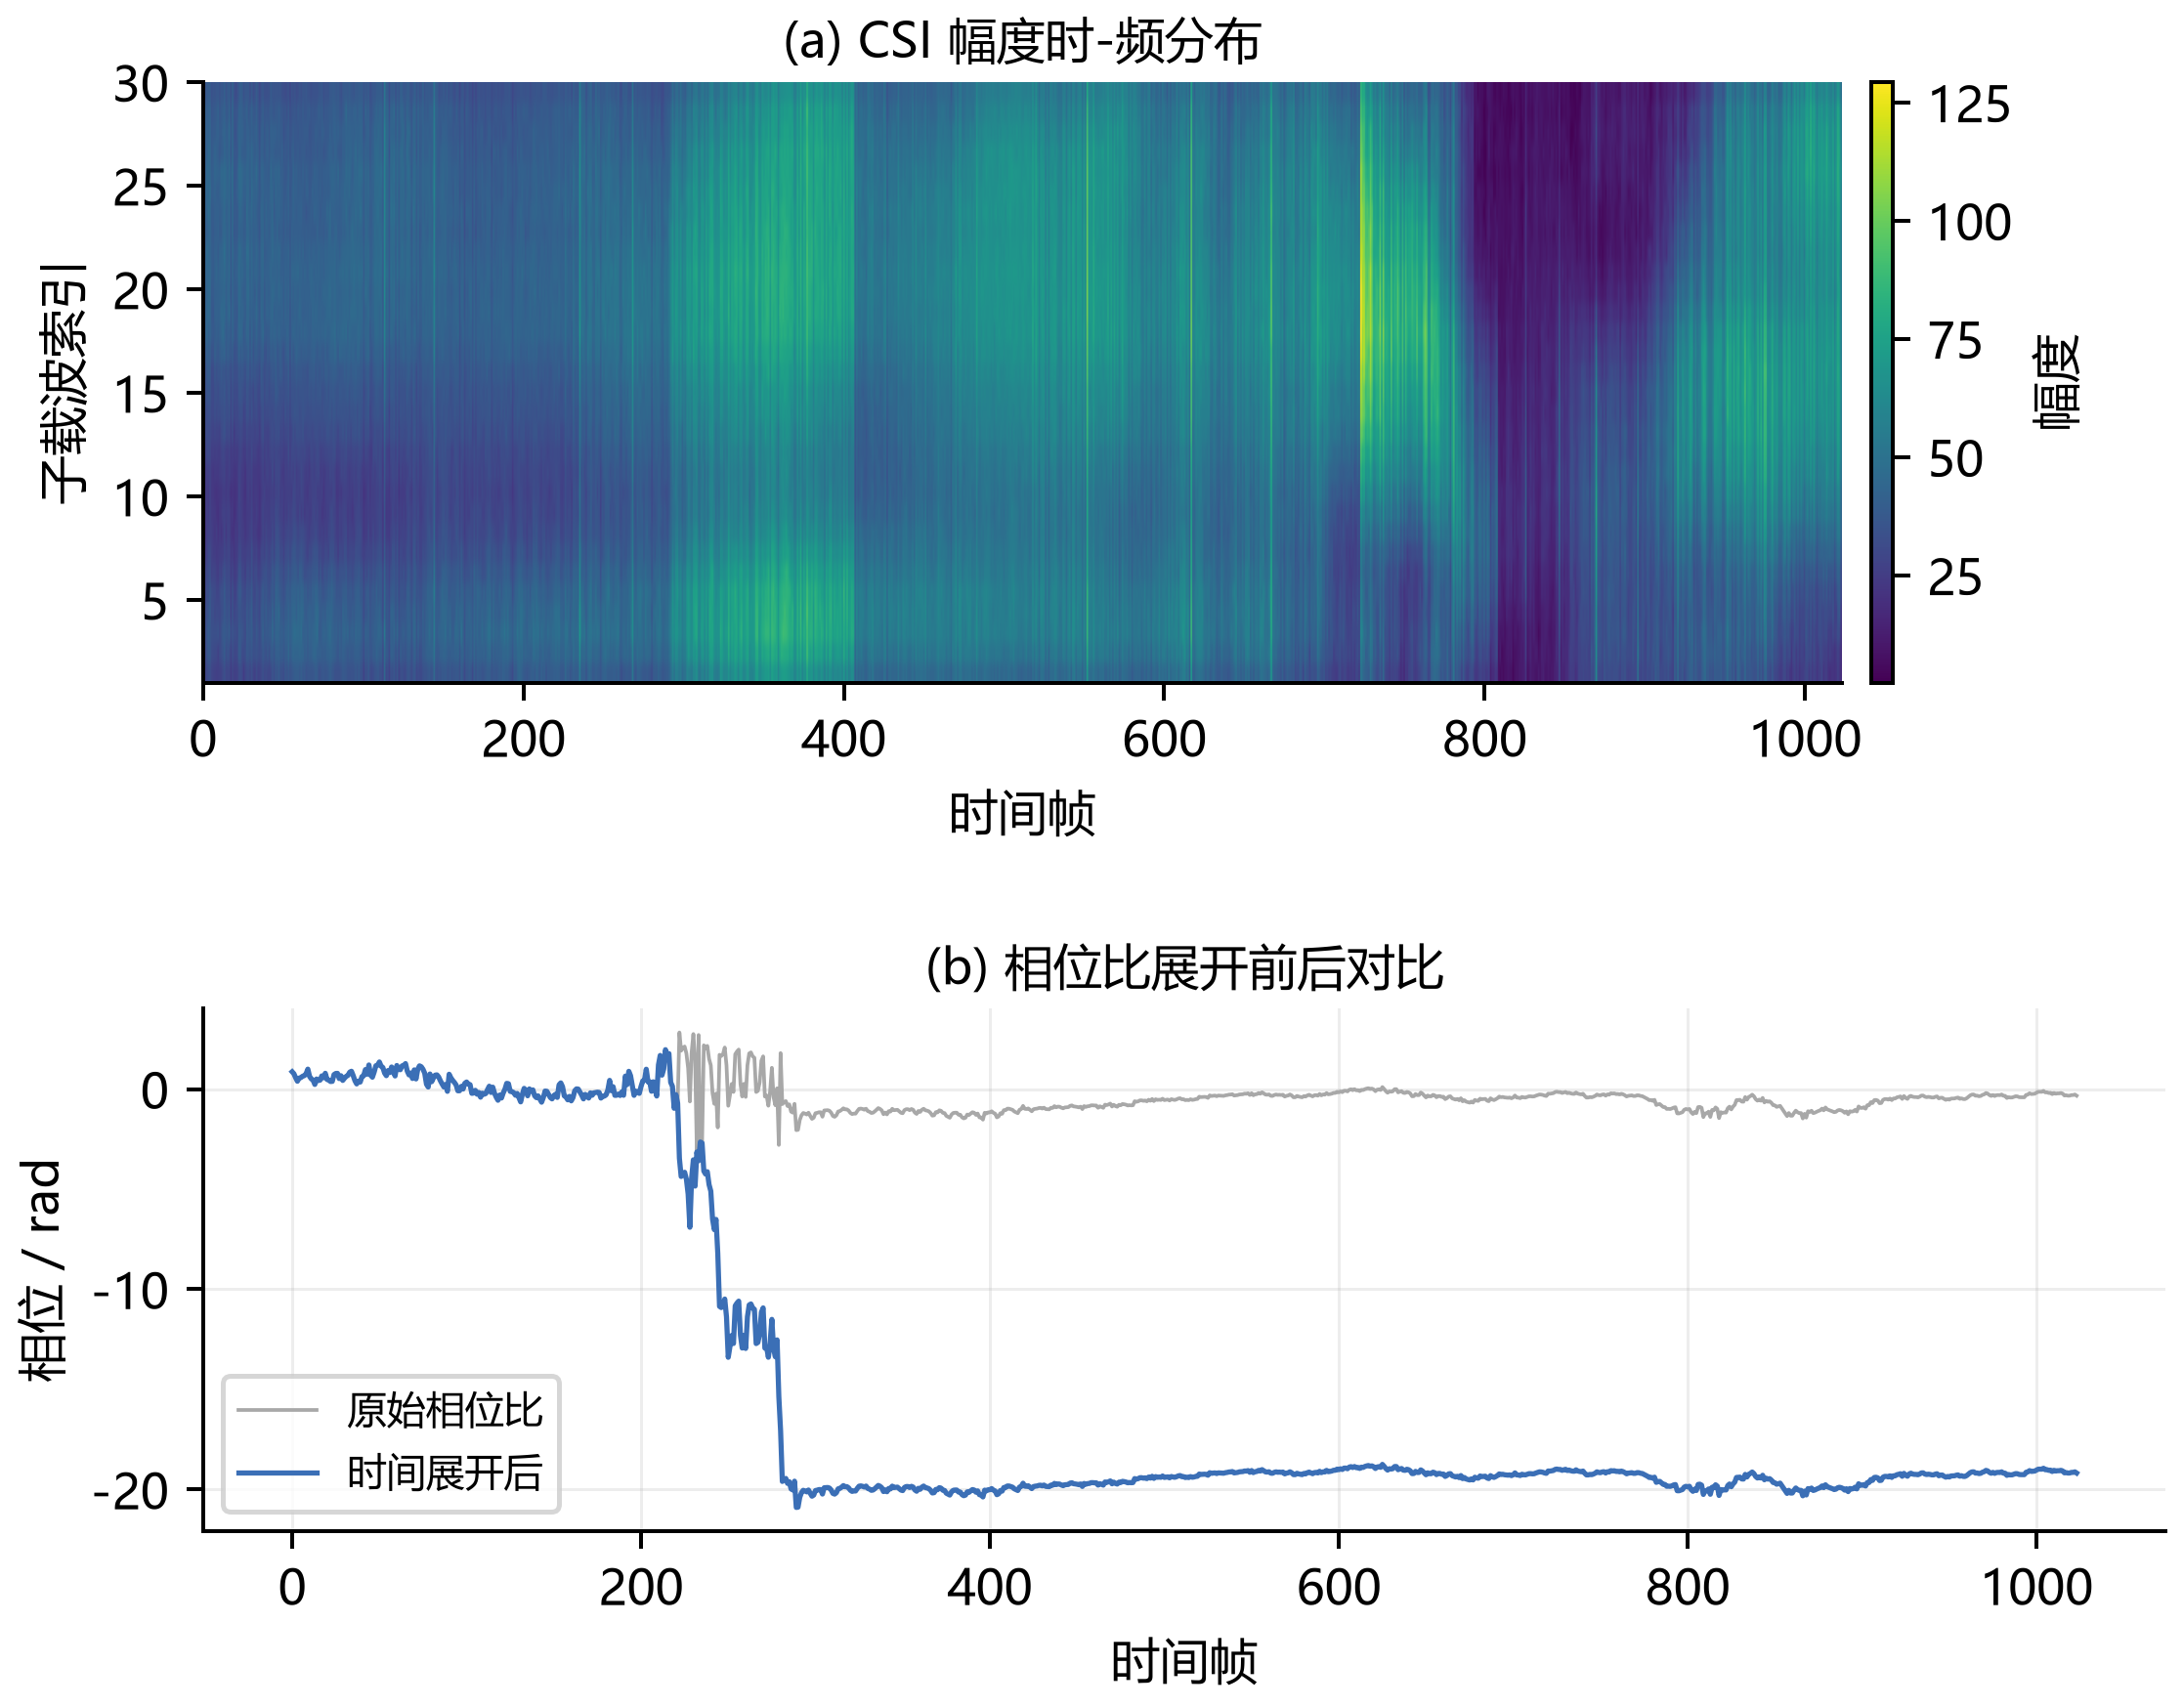
\includegraphics[width=0.92\textwidth]{figures/csi_signal_example.png}
\caption{真实 CSI 样例及接收天线相位比的时间展开效果}
\label{fig:csi_signal_example}
\end{figure}

\section{滑动窗口组织}
原始 CSI 文件通常包含连续采集得到的一整段时间序列，不同文件的长度可能存在差异。为了统一处理长序列，本文采用长度为 512、步长为 256 的滑动窗口切分相位比序列。设窗口长度为 $L$、滑动步长为 $P$，则第 $k$ 个窗口可表示为
\begin{equation}
W_k=\left[\tilde{\theta}_{kP},\tilde{\theta}_{kP+1},\ldots,\tilde{\theta}_{kP+L-1}\right].
\end{equation}

窗口化的作用是将长 CSI 文件分解为若干局部时间片段，使后续特征统计能够同时覆盖局部变化和整段采集过程。本文最终分类单位仍为完整原始文件，而不是单个窗口。这样能够避免仅凭短时间片段判断整体脊柱姿态，同时保留同一文件内多个窗口所包含的时间变化信息。

窗口长度决定单个局部片段覆盖的时间范围。窗口过短时，统计量容易受到瞬时噪声影响，难以反映相对稳定状态；窗口过长时，局部变化可能被过度平滑，并增加不同长度序列之间的处理差异。滑动步长则决定相邻窗口的重叠程度：较小步长可以提高时间覆盖的连续性，但会产生更多高度相关的窗口。因此，窗口参数应综合考虑信号持续时间、局部稳定性和计算开销，并且必须在验证集上选择，不能根据测试集结果反向调整。

对于长度不足一个完整窗口的序列，可以采用丢弃、补齐或变长统计等处理方式。不同策略会改变有效样本信息，因此应在训练和检测阶段保持一致，并记录短序列处理规则。对于长序列，窗口化只用于组织特征计算，同一原始文件产生的窗口始终属于同一数据子集，避免重叠片段跨越训练集与测试集。

\section{文件级统计特征}
在完成窗口化后，系统将同一原始文件产生的全部窗口重新聚合，并对每个相位比特征计算统计量。当前每一时间帧整理得到 180 个相位比特征；对每个特征计算 9 组统计量，包括均值、标准差、10\% 分位数、中位数、90\% 分位数、相邻帧差分绝对值均值、相邻帧差分标准差、相位正弦均值和相位余弦均值。因此，每个原始文件最终形成
\begin{equation}
180\times 9=1620
\end{equation}
维文件级特征向量。

这些统计量分别描述相位比序列的整体水平、波动程度、分布位置、动态变化和周期性信息。分位数统计可降低少量异常帧对特征的影响；差分统计刻画姿态相关扰动在时间上的变化强度；正弦和余弦统计保留相位特征的周期性质。通过文件级聚合，系统将连续 CSI 信号转化为固定长度向量，为 ExtraTrees 分类器提供稳定输入。

从特征含义看，均值和分位数主要描述序列的位置与分布范围，标准差描述整体离散程度，差分特征描述相邻时刻变化强度。由于相位属于周期变量，直接对展开后的数值求均值可能受到累计周期变化影响，正弦均值和余弦均值则可以从圆周统计角度表达相位集中方向。多类统计量共同使用，使固定长度向量同时包含分布、动态和周期信息。

\section{特征处理的稳定性原则}
为了保证分类结果能够被正确解释，特征处理流程需要满足一致性、稳健性和隔离性三个原则。一致性要求训练、验证和检测阶段采用完全相同的天线顺序、子载波顺序、窗口规则和统计量定义；稳健性要求对分母接近零、非有限数值、异常跳变和长度不足等情况进行统一处理；隔离性要求所有依赖数据分布的处理参数仅从训练集获得，测试集不得参与阈值选择或特征筛选。

此外，固定长度表示虽然便于传统分类器处理，但会压缩原始时间顺序信息。统计聚合适合描述相对稳定姿态的总体规律，却可能无法完整表达快速、短暂或顺序相关的动作过程。因此，特征表示必须与研究对象匹配：对于稳定状态，可以强调分布和变化强度；对于复杂动作，则可能需要保留更完整的时序结构。

\section{本章小结}
本章建立了从多维复数 CSI 到文件级统计表示的处理过程。首先分析人体姿态通过多径传播影响信道响应的基本机理，并说明原始相位中的公共偏移和链路误差；随后利用接收天线复数比值构造相对相位，通过时间展开和滑动窗口组织连续序列；最后使用分布、差分和周期统计量形成固定长度特征。上述步骤的核心目标是在保留姿态相关差异的同时，提高不同处理阶段的数据一致性和表示稳定性。
